\documentclass[a4paper]{article}

\usepackage{graphicx} 
\usepackage[english]{babel}
\usepackage{graphicx}
\usepackage{float}
\usepackage{logicproof}
\usepackage{amssymb}
\usepackage[a4paper,top=3cm,bottom=2cm,left=2cm,right=2cm,marginparwidth=1.75cm]{geometry}

\begin{document}

\begin{titlepage}
    \newcommand{\HRule}{\rule{\linewidth}{0.5mm}}
    \center

    \textsc{\LARGE Delft University of Technology}\\[1cm]

    \textsc{\Large Reasoning \& Logic}\\[0.2cm]
    \textsc{\large CSE1300}\\[1cm]
    \HRule \\[0.8cm]
    { \huge \bfseries Assignment: TA-check 3}\\[0.7cm]
    \HRule \\[2cm]
    \large
    \emph{Authors:}\\
    Joris Rijs (5880998) \& Sebastiaan Beekman (5885116)\\[1.5cm]
    {\large \today}\\[5cm]
    
\includegraphics[width=0.6\textwidth]{images/TU_delft_logo.jpg}\\[1cm]
    \vfill
\end{titlepage}

\newpage
\tableofcontents

\newpage
\section{Question 1}

\newpage
\section{Question 2. First steps in recursive functions}
\textbf{(a). Consider the following recursive function f(n). List the first 7 values of f(n), so for n = 0 to n = 6}
\begin{center}
    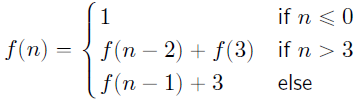
\includegraphics[width=0.6\textwidth]{images/2a.png}\\[1cm]
\end{center}

\begin{itemize}
    \item f(0) = 1
    \item f(1) = f(0) + 3 = 4
    \item f(2) = f(1) + 3 = 7
    \item f(3) = f(2) + 3 = 10
    \item f(4) = f(2) + f(3) = 17
    \item f(5) = f(3) + f(3) = 20
    \item f(6) = f(4) + f(3) = 27
\end{itemize}
\ \\

\textbf{(b). Consider the following recursive function g(n). List the first 7 values of g(n), so for n = 0 to n = 6}
\begin{center}
    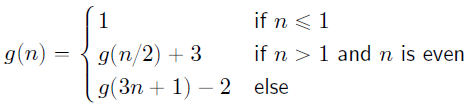
\includegraphics[width=0.6\textwidth]{images/2b.png}\\[1cm]
\end{center}

\begin{itemize}
    \item g(0) = 1
    \item g(1) = 1
    \item g(2) = g(1) + 3 = 4
    \item g(3) = g(10) - 2 = 12
    \item g(4) = g(2) + 3 = 7
    \item g(5) = g(16) - 2 = 11
    \item g(6) = g(3) + 3 = 15
    \item g(8) = g(4) + 3 = 10
    \item g(10) = g(5) + 3 = 14
    \item g(16) = g(8) + 3 = 13
\end{itemize}

\newpage

\textbf{(c). Formulate a recursive function hpnq that computes the number of odd digits in a number}
\begin{center}
    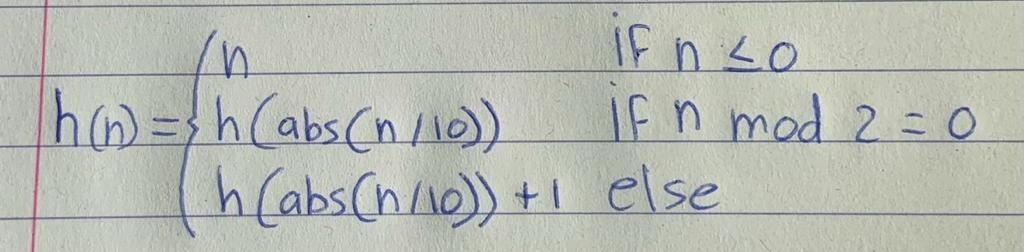
\includegraphics[width=0.6\textwidth]{images/2c.jpeg}\\[1cm]
\end{center}

\newpage

\section{Question 3. A first induction proof}
Prove the following theorem using mathematical induction:
\textbf{Theorem.} For all integers n $\geq $ 1: $\sum^n_{i=1}{\frac{1}{i(i + 1)} = \frac{n}{n + 1}}$.\\
P(n) = $\sum^n_{i=1}{\frac{1}{i(i + 1)} = \frac{n}{n + 1}}$\\
\textbf{Proof.} We will prove this theorem by induction\\
\textbf{Base case:} Consider the case n = 1. P(1) = $\sum^1_{i=1}{\frac{1}{i(i + 1)} = \frac{1}{1 + 1}}$. Since each side of the equation is equal to $\frac{1}{2}$, this is true.\\
\textbf{Inductive step:} Let k $\geq$ 2 be arbitrary. Assume that P(k) is true. We want to show that P(k + 1) is true. P(k + 1) is the statement $\sum_{i=1}\limits^{k+1}{\frac{1}{i(i + 1)} = \frac{(k+1)}{(k+1) + 1}}$. But, we can compute that\\
$\sum_{i=1}\limits^{k+1}{\frac{1}{i(i + 1)} = (\sum_{i=1}\limits^{k}{\frac{1}{i(i + 1)}}) + \frac{1}{(k+1)((k+1) + 1)}}$.\\
Since P(k) is true, we can replace the first sum with $\frac{k}{k + 1}$.\\
This gives us $\frac{k}{k + 1} + \frac{1}{(k+1)((k+1) + 1)} = \frac{k + 1}{(k + 1) + 1}$\\
which is what we wanted to show. This completes the induction.\\

\newpage

\section{Question 4. Satisfiability of propositions}
\textbf{(a).} Explain when a proposition is satisfiable and how you can show that a proposition is satisfiable\\
A proposition is satisfiable when there exsists a truth assignment that makes the proposition true. This can be shown by using a truth table.\\

\textbf{(b).} What property does a proposition that is not satisfiable have?\\
A proposition that is not satisfiable has the property that no truth assignment can make the proposition true, thus a contradiction.\\

\textbf{(c).} How can you show that a proposition is not satisfiable?\\
A proposition is not satisfiable when it is a contradiction.\\

\textbf{(d).} For each of the following domains and propositions, show that they are either satisfiable or not. If
the proposition is satisfiable, show this using a formal structure using all elements in the domain. If
the proposition is not satisfiable, explain that is it not satisfiable using the method described in your
answer of c.\\

\begin{center}
    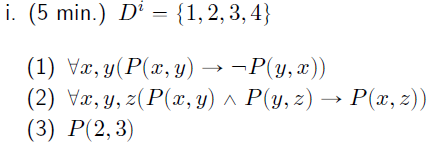
\includegraphics[width=0.6\textwidth]{images/4d1.png}\\[1cm]
\end{center}
Structure I with domain $D^i = \{1,2,3,4\}$ is satisfiable.

\begin{center}
    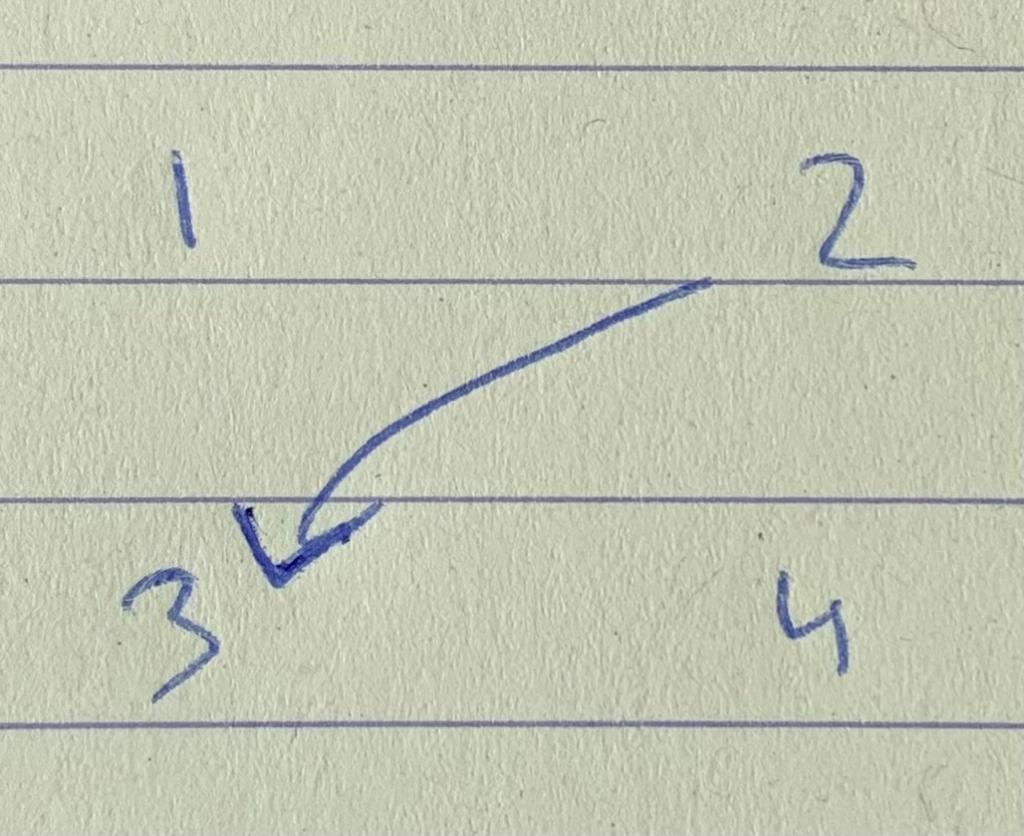
\includegraphics[width=0.6\textwidth]{images/4d1a.jpeg}\\[1cm]
\end{center}

\newpage

\begin{center}
    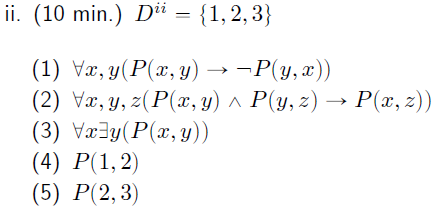
\includegraphics[width=0.6\textwidth]{images/4d2.png}\\[1cm]
\end{center}
Structure II with domain $D^{ii} = \{1,2,3\}$ is not satisfiable due to predicate 3.

\newpage

\section{Question 5. Revision}
\textbf{(a).} Consider the following argument written in propositional logic. If it is invalid provide a counterexample and explain how it shows the argument is invalid. If it is valid, prove it.\\
\begin{center}
    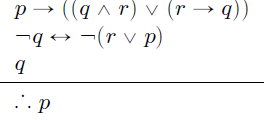
\includegraphics[width=0.6\textwidth]{images/5a.png}\\[1cm]
\end{center}

\begin{displaymath}
    \begin{array}{|c c c|c|c|c|c|c|c|}
        p & q & r & p \rightarrow ((q \wedge r) \vee (r \rightarrow q)) & \wedge & \neg q \leftrightarrow \neg (r \vee p) & \wedge & q & p \\
        \hline
        0 & 0 & 0 & 1                                                   & 1      & 1                                      & 1      & 0 & 0 \\
        0 & 0 & 1 & 1                                                   & 1      & 0                                      & 0      & 0 & 0 \\
        0 & 1 & 0 & 0                                                   & 1      & 0                                      & 0      & 0 & 1 \\
        0 & 1 & 1 & 1                                                   & 1      & 1                                      & 1      & 1 & 1 \\
        \hline
        1 & 0 & 0 & 1                                                   & 1      & 0                                      & 0      & 0 & 0 \\
        1 & 0 & 1 & 1                                                   & 0      & 0                                      & 0      & 0 & 0 \\
        1 & 1 & 0 & 1                                                   & 1      & 1                                      & 1      & 1 & 1 \\
        1 & 1 & 1 & 1                                                   & 1      & 1                                      & 1      & 1 & 1 \\
    \end{array}
\end{displaymath}

The last two situations of the truth table show that the argument is valid.\\

\newpage

\textbf{(b).} Consider the following argument written in predicate logic. Provide a counterexample in the form of a formal structure.\\
\begin{center}
    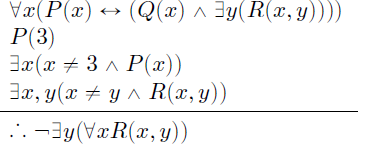
\includegraphics[width=0.6\textwidth]{images/5b.png}\\[1cm]
\end{center}

\begin{center}
    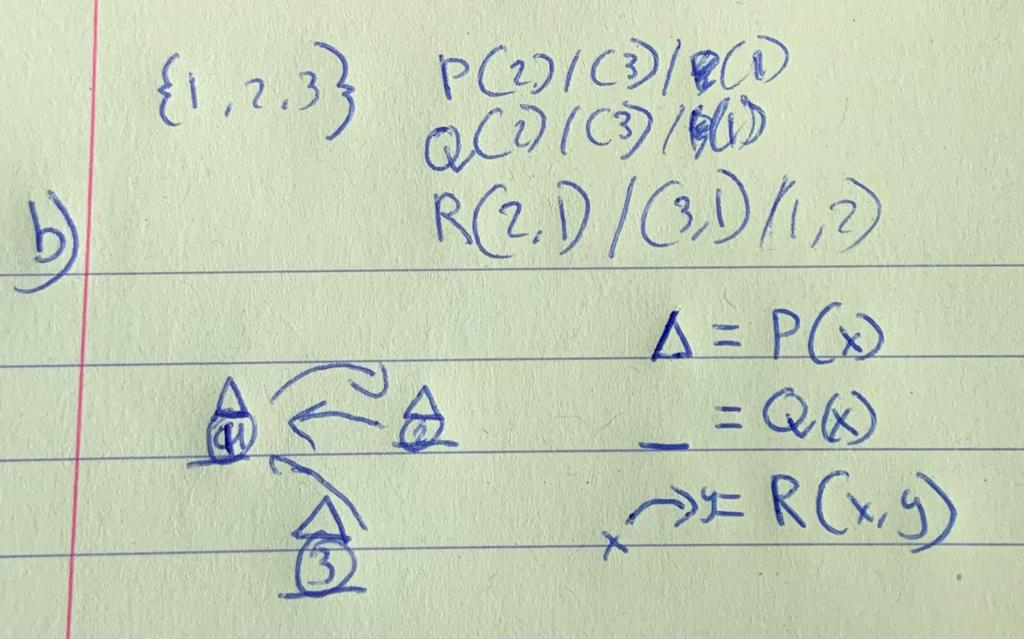
\includegraphics[width=0.6\textwidth]{images/5ba.jpeg}\\[1cm]
\end{center}

\newpage

\section{Question 6. Essay questions}
\textbf{(a).} In your own words, describe what a theorem prover such as Z3 does and why this tool can be useful.\\
Z3 theorem prover is a program that can analyse and prove theorems digitally. It can be useful because it can prove theorems that are difficult to prove by hand.\\

\textbf{(b).} In your own words, explain the idea and structure of an induction proof.\\
An induction proof is a proof that uses induction to prove a statement. It is structured by first proving the base case, then proving the inductive step.\\


\end{document}
